% Nome do capítulo
\chapter{Revisão Bibliográfica}
\label{cap:2}
\vspace{-1.9cm}

%Neste capítulo serão apresentados os principais conceitos e definições da literatura sobre \ac{RNA}, Deep Learning, classificação e localização de objetos.

\section{\textit{Machine Learning}}
\label{secao:2:1}
\vspace{-.6cm}

\textit{Machine Learning} ou Aprendizado de Máquina é um campo de estudo cada vez mais recorrente na área de tecnologia. Em uma definição alternativa, pode-se dizer que ``Aprendizado de Máquina é uma área de Inteligência Artificial cujo objetivo é o desenvolvimento de técnicas computacionais sobre o aprendizado bem como a construção de sistemas capazes de adquirir conhecimento de forma automática'' \cite{monard-2003}. Entre as principais aplicações de Aprendizado de máquina, pode se destacar o reconhecimento de padrões, classificação de imagens e a mineração de dados. 

\citeonline{monard-2003} define ainda que o aprendizado de máquina pode ser supervisionado ou não-supervisionado. Quando falamos do primeiro caso, queremos dizer que o algoritmo recebe um conjunto de dados na entrada, processa esses dados e retorna uma saída. Essa saída é comparada com um valor previamente associado à entrada, comumente conhecido como rótulo. Já no aprendizado não-supervisionado, as entradas não possuem rótulo algum, cabendo ao algoritmo fazer a distinção das diversas entradas. Geralmente nesses casos, é necessária uma análise posterior à execução do algoritmo para se entender os resultados obtidos.

O aprendizado supervisionado se divide em dois grupos menores: classificação e regressão. \citeonline{santos-2012} define que quando o problema possui um conjunto discreto de saídas e o objetivo é atribuir a qual dessas saídas a entrada pertence, se trata de um problema de classificação. \citeonline{santos-2012} define ainda que quando o objetivo é prever uma saída de valor contínuo pra uma entrada, se trata de um problema de regressão.

As seções \ref{subsecao:2:1:1} e \ref{subsecao:2:1:2} irão definir melhor esses conceitos.

\vspace{-1cm}
\subsection{Regressão}
\label{subsecao:2:1:1}

Como definido anteriormente, o problema de regressão consiste em calcular para cada entrada uma saída que possua um valor contínuo. \citeonline{dosualdo-2003} define que a regressão consiste em fazer uma relação entre os atributos $X={x_1, x_2,..., x_n}$ - onde $X$ é o conjunto de entrada e cada $x_i$ é um atributo numérico ou quantitativo - e $Y$, tal que $Y$ é um atributo ou um conjunto de atributos meta. \citeonline{apte-1997} define essa relação através da equação \ref{eq:eq1}:

\begin{equation}
\label{eq:eq1}
	Y = f(x_1, x_2,..., x_n)
\end{equation}

A relação entre o(s) atributo(s) $X$ e o(s) atributo(s)-meta $Y$ alcançada como resultado de um algoritmo de regressão é chamado de modelo. Após a definição do modelo é importante fazer uma avaliação para dizer o quão confiável será a predição gerada pelo modelo. Existem diversas funções usadas na avaliação dos algoritmos de regressão, e uma das mais comuns é o \ac{MLS} que é definido pela equação \ref{eq:eq2}:

\begin{equation}
\label{eq:eq2}
	E = \sum_{i = 0}^{N}(Y_i - f(X)_i)^2
\end{equation}

Onde $E$ é o erro, $N$ é o tamanho do conjunto de amostras, $Y_i$ é o valor esperado do atributo-meta e $f(X_i)$ é o resultado do modelo para a entrada $X_i$.

Alguns exemplos de problemas de regressão são: 

\begin{enumerate}
	\item Predizer o percentual de gordura que uma pessoa possui no corpo, recebendo como entrada atributos como altura, idade, peso, sexo \cite{dosualdo-2003}.
	\item Predizer o preço de um imóvel baseado em atributos como o tamanho, número de cômodos, número de quartos, etc. \cite{pereira-2012}.
\end{enumerate}

Uma grande limitação nos métodos de regressão é que eles em sua maioria solucionam problemas que possuem apenas um atributo-meta. Porém, os métodos de regressão baseados em \ac{RNA} podem retornar múltiplos resultados. Esse termo será definido na Sessão \ref{secao:2:2}.

\subsection{Classificação}
\label{subsecao:2:1:2}

Como definido anteriormente, o problema de classificação consiste em um problema de predição quando as saídas são discretas.

\section{Redes Neurais Artificiais}
\label{secao:2:2}

As \ac{RNA} são uma das principais técnicas de aprendizagem de máquina e podem ser implementadas tanto para problemas supervisionados, quanto não-supervisionados. \citeonline{jost-2015} definiu as \ac{RNA}s da seguinte forma:

\begin{citacao}
	As \ac{RNA}s possuem inspiração nas redes neurais biológicas, constituídas de neurônios separados por camadas, que processam informações e estão conectados via pesos sinápticos, sendo na maioria das vezes sistemas adaptativos que modificam sua estrutura através de informações, que fluem pela rede durante a etapa de aprendizado \cite{jost-2015}.
\end{citacao}

Além disso, é importante mencionar que em uma rede neural, existem duas camadas em particular que são muito importantes: a primeira camada, que é a camada de entrada de dados, e a última camada que é a camada de saída. Existem dois tipos de \ac{RNA}s: as redes \textit{feed forward}, que processamento sempre flui da entrada para a saída, e as redes recorrentes, que os dados fluem nos dois sentidos.

A \ac{RNA} \textit{feed forward} mais básica que existe é a perceptron, composta apenas por um conjunto de neurônios de entrada e um único neurônio de saída. A Equação \ref{eq:eq3} representa a fórmula de um perceptron, onde $n$ é o número de entradas, $W_i$ são os respectivos pesos de cada entrada, $X_i$ são as entradas e $B$ é o Bias do neurônio.

\begin{equation}
Y=\Big(\sum_{i=1}^{n}{(W_i \times X_i)}\Big) - B
\label{eq:eq3}
\end{equation}

Uma rede percepron não é uma arquitetura de redes neurais artificiais muito poderosa, mas deu base para outras arquiteturas mais robustas. A principal delas, é o Perceptron Multi-Camadas.

\subsection{\textit{Multi-Layer Perceptron}}
\label{subsecao:2:2:2}


A rede Perceptron Multicamadas ou \ac{MLP} são baseadas nos Perceptrons simples, como mencionado anteriormente. A diferença, porém, é que elas trabalham com mais camadas do que simplesmente as camadas de entrada e saída. Geralmente elas possuem uma ou duas camadas intermediárias às camadas externas. Essas camadas intermediárias, também são chamadas de camadas ocultas e servem para conferir uma robustez maior ao método.

Uma outra diferença das \ac{MLP}s para as perceptrons comuns é a equação para calcular a saída de cada neurônio. Nas redes \ac{MLP}s, a equação utilizada é a função sigmóide. A Equação \ref{eq:eq4} descreve a fórmula da função sigmóide.

\begin{equation}
Y= \dfrac{1}{1+e^z}
\label{eq:eq4}
\end{equation}

Onde $z$ é descrito pela Equação \ref{eq:4}:

\begin{equation}
Z_{(i+1) j} = \Big(\sum_{k=1}^{n} (W_{i k}\times X_{i k})\Big)-B_j
\label{eq:4}
\end{equation}

Onde $i$ é o número da camada, $j$ o neurônio de destino, $k$ o neurônio de origem, $W$ é o peso e $X$ a entrada.

Como foi dito anteriormente, a \ac{MLP} trabalha com aprendizado supervisionado, isso quer dizer que os dados que ela opera são rotulados, e tem uma saída esperada. Quando as entradas são processadas e os resultados das saídas são calculados, eles são comparados com os valores esperados pelos rótulos e é gerado a função de erro quadrático, definida pela Equação \ref{eq:5}:

\begin{equation}
E=\dfrac{1}{2}\times \sum_{i=1}^{n}(Y_i-O_i)^2
\label{eq:5}
\end{equation}

Onde $n$ é o número de saídas, $i$ é qual saída calculada, $Y$ são as saídas da rede e $O$ são as saídas esperadas.

Sabendo-se disso, o objetivo para melhorar a precisão da \ac{MLP} é minimizar o valor da função erro, ou seja, tornar as saídas da rede o mais próximo possível das saídas esperadas. Para tanto, é utilizado o método de retropropagação de erro que reajusta os pesos da rede de acordo com os valores obtidos usando a descida de gradiente.

\citeonline{arnold-2011} define que aumentar o número de camadas em um \ac{MLP} não garante uma melhoria dos resultados, pois a descida de gradiente pode chegar a um mínimo local. Além disso, o aumento do número de camadas implica em um tempo muito maior de processamento. Para lidar com esse problema surge o \emph{Deep Learning}, uma arquitetura avançada com múltiplas camadas, que soluciona a dificuldade que as redes neurais possuem ao lidar com dados de alta dimensionalidade \cite{arnold-2011}.

\section{\textit{Deep Learning}}
\label{secao:2:3}


A principio não parecia ser viável manipular arquiteturas profundas de redes neurais. Porém, de acordo com \citeonline{deng-2014} surgiu um algoritmo de aprendizado não-supervisionado que conseguiu aliviar empiricamente as dificuldades de otimização em arquiteturas profundas. Esse algoritmo é a \ac{DBN}, um modelo generativo profundo composto de uma camada visível e várias camadas ocultas compostas por uma pilha de \ac{RBM}s.

\citeonline{deng-2014} definem ainda que o aprendizado nas \ac{DBN}s é feito por um algoritmo guloso que ajustas os pesos camada-por-camada com uma complexidade linear ao tamanho e à profundidade da rede. E uma relação inesperada entre as \ac{DBN}s e as \ac{MLP}s surgiu quando descobriu-se que ao utilizar os pesos de uma \ac{DBN} com arquitetura correspondente, você consegue inicializar os pesos de uma \ac{MLP} de forma a produzir melhores resultados do que utilizando pesos aleatórios.

Uma segunda alternativa para trabalhar com aumento de camadas é o empilhamento de auto-codificadores. O empilhamento de auto-codificadores consiste basicamente em inserir na saída de uma rede neural uma segunda rede neural que pra cada entrada produz uma saída específica e retreinar a nova rede neural utilizando o algoritmo de retropropagação de erro \cite{deng-2014}.

\subsection{Redes Neurais Convolucionais}
\label{subsecao:2:3:1}


As \ac{CNN} são um modelo específico de \textit{Deep Learning} muito utilizados em aplicações de visão computacional e aplicações de reconhecimento de imagens. De acordo com \citeonline{ferreira-2017}, as \ac{CNN}s utilizam matrizes para processar as entradas de dados, sendo essas matrizes unidimensionais para sinais e sequências, bidimensionais para imagens e tridimensionais para imagens volumétricas e vídeos. 

Ao contrário das \ac{RNA}s tradicionais (como \ac{MLP}), as \ac{CNN}s não necessariamente ligam todos os neurônios na camada de origem a todos os neurônios da camada de destino. \citeonline{ferreira-2017} define que existem três tipos comuns de camadas utilizadas nas redes neurais convolucionais: as camadas de convolução, camadas de pooling e camadas completamente conexas.

A ideia da camada de convolução, é de que cada neurônio recebe como entrada neurônios próximos e tem por objetivo criar mapas e filtros. \citeonline{ferreira-2017} define que em aplicações de reconhecimento de objetos, por exemplo, é comum as primeiras camadas de convolução detectarem bordas ou manchas que seriam as características mais básicas da imagem. As camadas de convolução mais profundas, detectam outras características mais específicas.

As camadas de pooling são utilizadas para reduzir a dimensão de dados vindo das camadas de convolução, consequentemente reduzindo o custo computacional \cite{ferreira-2017}. Um exemplo seria receber como entrada uma matriz 4x4 e enviar para a próxima camada uma matriz 2x2 escolhendo um representante de cada quatro da matriz de entrada para a matriz de saída, sendo que esse representante é determinado por alguma propriedade específica. As propriedades mais utilizadas são a de máximo e de média \cite{ferreira-2017}.

Por fim, as camadas completamente conexas são exatamente iguais às redes MLP e é comum utilizá-las no final da rede para conectar à saída. Seu acréscimo no final é importante pois faz a ligação de todos os filtros \cite{ferreira-2017}. As arquiteturas de \ac{CNN}s geralmente intercalam algumas camadas de convolução com uma camada de pooling e com duas camadas completamente conexas ao final.

\section{Imagem}
\label{secao:2:4}

\citeonline{torres-2006} definem uma imagem Î como sendo um par ($D_i$,$\vec{I}$) onde:
%\vspace{-1.9cm}

\begin{itemize}
	\item $D_i$ é um conjunto finito de \ac{Pixels};
	\item $\vec{I}$:$D_I$ $\mapsto $${R}$$^n$ é uma função que atribui para cada \textit{pixel} p em $D_i$ um vetor $\vec{I} \in R^n$ (quando uma cor RGB é atribuída a cada \textit{pixel}, por exemplo, podemos dizer que $\vec{I} \in R^3$).
	
\end{itemize}
%\vspace{-1.9cm}

Uma imagem digital pode ser considerada como a representação numérica da luz refletida em um determinado ponto representado no espaço. No caso de uma imagem em tons de cinza, a luz é amostrada em um ponto \textit{(X,Y)} e quantizada para um valor inteiro. Sendo colorida, a luz é quantizada para os valores de vermelho ou \textit{red}(R), verde ou \textit{green}(G) e azul ou \textsl{blue}(B), tendo então três componentes. Cada elemento amostrado é considerado um pixel da imagem. Sendo assim, \textit{$D_i$} representa a posição de cada ponto amostrado enquanto o vetor \textit{$\vec{I}$}, é uma função que mapeia cada pixel \textit{p} da imagem, em um valor real para todas as suas componentes, no caso R, G e B.



%%%%%%%%%%%%%%%%%%% Formato para a inserção de figuras

%  \begin{figure}[H]
  % Alterar espaçamentos antes e depois do caption
%  \setlength{\abovecaptionskip}{0pt}
%  \setlength{\belowcaptionskip}{0pt}
  % Caption
%  \caption[Principais componentes de WiNoCs]{Principais componentes de WiNoCs}
%  \centering
%  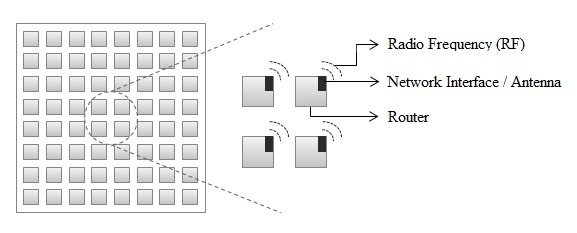
\includegraphics[width=.85\textwidth]{imagem/winoc.jpg}
  % Caption centralizada
%  \captionsetup{justification=centering}
%  \captionfont{\small{\textbf{\\Fonte: \cite{OliveiraIadis:2011}}}}	
%  \label{fig:ComponentesWiNoC}
%  \end{figure}


%%%%%%%%%%%%%%%%%%%%%%%%%% Modelo para inserir gráficos

%\begin{grafico}[H]
  % Alterar espaçamentos antes e depois do caption
%  \setlength{\abovecaptionskip}{5pt}
%  \setlength{\belowcaptionskip}{0pt}
  % Caption
%  \caption[Percentual de pacotes enviados]
%	  {Percentual de pacotes enviados}
%  \centering
%  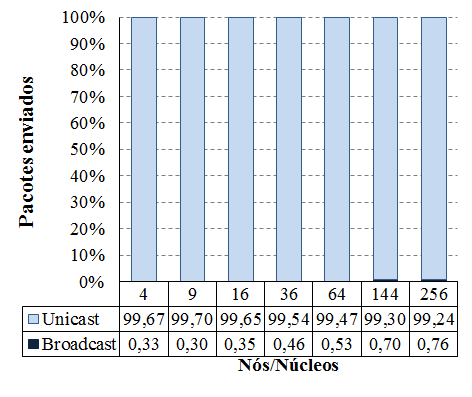
\includegraphics[width=.48\textwidth]{imagem/graficos/grafico_pacotes_enviados_bt.png}
  % Caption centralizada
%  \captionsetup[grafico]{justification=centering}
  % Fonte
%  \captionfont{\small{\textbf{\\Fonte: Dados da pesquisa}}}
%  \end{grafico}


%\begin{grafico}[H]
  % Alterar espaçamentos antes e depois do caption
%  \setlength{\abovecaptionskip}{5pt}
%  \setlength{\belowcaptionskip}{0pt}
  % Caption
%  \caption[Resultados da carga de trabalho 1]
%	  {Resultados da carga de trabalho 1}
%  \centering
%  \subfloat[Enviados]
%      {\label{graf:enviados_bt}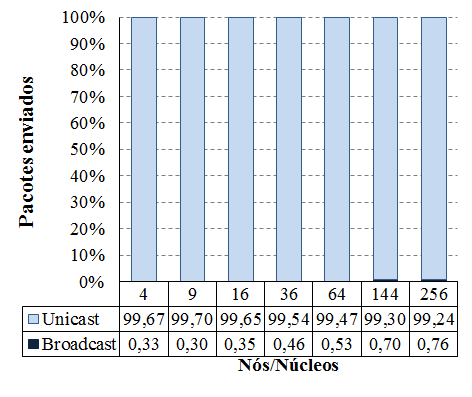
\includegraphics[width=.48\textwidth]{imagem/graficos/grafico_pacotes_enviados_bt.png}} \quad
%  \subfloat[Perdidos]
%      {\label{graf:perdidos_bt}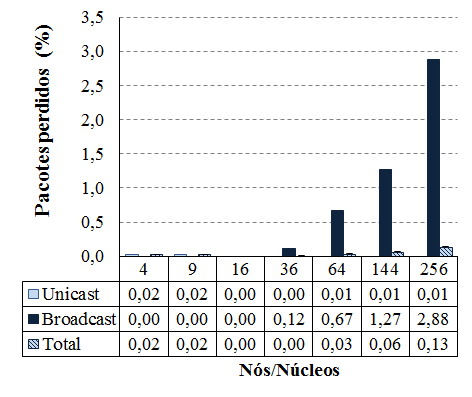
\includegraphics[width=.48\textwidth]{imagem/graficos/grafico_pacotes_perdidos_bt.png}} \quad
%  \subfloat[Taxa de injeção]
%      {\label{graf:injecao_bt}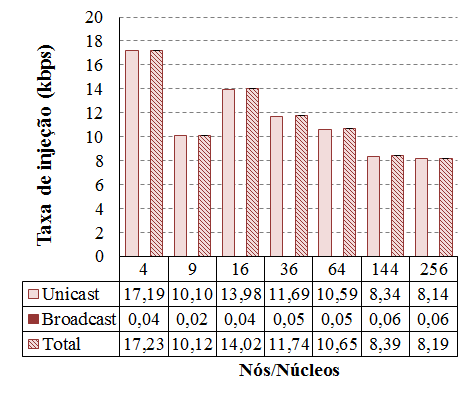
\includegraphics[width=.48\textwidth]{imagem/graficos/grafico_taxa_injecao_bt.png}} \quad
%  \subfloat[Vazão]
%      {\label{graf:vazao_bt}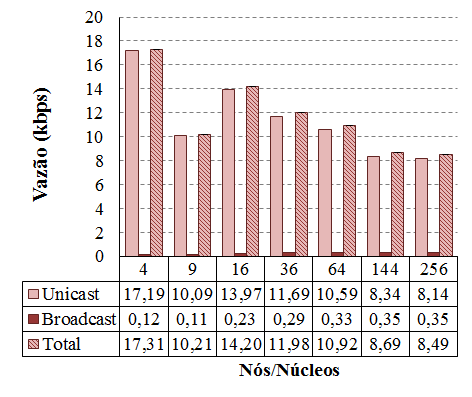
\includegraphics[width=.48\textwidth]{imagem/graficos/grafico_vazao_bt.png}}
  % Caption centralizada
%  \captionsetup[grafico]{justification=centering}
  % Fonte
%  \captionfont{\small{\textbf{\\Fonte: Dados da pesquisa}}}
%  \label{graf:quad}
%  \end{grafico}

%%%%%%%%%%%%%%%%%%%%%%%% Exemplo de criação de tabelas

   % Tabela
%  \begin{table}[H]
%    \centering
%    \footnotesize
    % Alterar espaçamentos antes e depois do caption
%    \setlength{\abovecaptionskip}{0pt}
%    \setlength{\belowcaptionskip}{0pt}
    % Caption
%    \caption[Parâmetros definidos por classe]{Parâmetros definidos por classe}
%    \label{tab:classesNas}
    % Conteúdo da tabela
%    \begin{tabular}{c|c|c|c|c|c|c|c}
%	\hline \hline
%	\textit{Benchmark} &	Parâmetro &	Classe S &	Classe W &	Classe A &	Classe B &	Classe C &	Classe D \\ 
%	\hline \hline
% 	BT & \textit{Grid}	& $12^3$	& $24^3$ 	& $64^3$	& $102^3$ 	& $162^3$	& $408^3$ \\ 
%	CG & Linhas		& 1400		& 7000 		& 14000 	& 75000 	& 150000 	& 1500000 \\ 
%	EP & Pares 		& $2^{24}$	& $2^{25}$	& $2^{28}$	& $2^{30}$	& $2^{32}$	& $2^{36}$ \\
%	FT & \textit{Grid}	& $64^3$	& $128^2*32$	& $256^2*128$	& $512*256^2$	& $512^3$	& $2048*1024^2$ \\ 
%	IS & Chaves		& $2^{16}$	& $2^{20}$	& $2^{23}$	& $2^{25}$	& $2^{27}$	& $2^{31}$ \\ 
%	LU & \textit{Grid}	& $12^3$	& $33^3$	& $64^3$	& $102^3$	& $162^3$	& $408^3$ \\
%	MG & \textit{Grid}	& $32^3$	& $128^3$	& $256^3$	& $256^3$	& $512^3$	& $1024^3$ \\ 
%	SP & \textit{Grid}	& $12^3$	& $36^3$	& $64^3$	& $102^3$	& $162^3$	& $408^3$ \\
%	\hline \hline
%    \end{tabular}
    % Fonte
%    \captionfont{\small{\textbf{\\Fonte: Adaptado de \cite{Nas:2011}}}}
%  \end{table}